% =============================
% Anhang
% =============================

\refstepcounter{chapter}
\chapter*{\thechapter. Anhang}
\addcontentsline{toc}{chapter}{\thechapter.\space Anhang}

\section{Glossar}

\begin{description}
    \item[\hypertarget{bra-ket-def}{}Bra-Ket-Schreibweise] 
    Notation zur Darstellung von Quantenzuständen, z.B. \( |0\rangle \) und \( |1\rangle \) für die Basiszustände eines Qubits.
    Diese repräsentieren einen Vektor in einem zweidimensionalen komplexen Vektorraum. Ket \( | \psi \rangle = \begin{pmatrix} \alpha \\ \beta \end{pmatrix} \) steht für einen Spaltenvektor, während Bra \( \langle \psi | = \begin{pmatrix} \alpha & \beta \end{pmatrix} \) für den Zeilenvektor steht.
    \\$|0\rangle$ steht für den zugehörigen Spaltenvektor $\begin{pmatrix} 1 \\ 0 \end{pmatrix}$ und $|1\rangle$ entspricht $\begin{pmatrix} 0 \\ 1 \end{pmatrix}$ \cite{bashiri2025quantencomputing}.
    
    \item[\hypertarget{fpga-def}{}Field-Programmable Gate Array-Schaltungen (feldprogrammierbare Gatter-Anordnung)]
    Integrierte Schaltkreise, die nach der Herstellung vom Benutzer programmiert werden können, um verschiedene logische Funktionen zu erfüllen.
    Sie bestehen aus einer Matrix von konfigurierbaren Logikblöcken und programmierbaren Verbindungsnetzwerken, die es ermöglichen, komplexe digitale Schaltungen zu erstellen.

    \item[\hypertarget{fourier-transform-def}{}Fourier-Transformation]
    Eine mathematische Methode zur Zerlegung eines Signals in seine Frequenzkomponenten.
    Sie wandelt ein zeitabhängiges Signal in ein frequenzabhängiges Signal um, indem sie das Signal als Summe von Sinusfunktionen unterschiedlicher Frequenzen und Amplitudendarstellt \cite{fourierTransform}.
    \begin{figure}[h!]
        \centering
        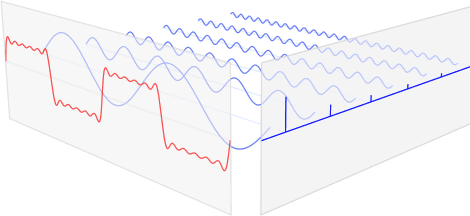
\includegraphics[width=0.4\textwidth]{images/fourier_transformation.png}
        \caption{Fourier-Transformation \cite{fourierTransform}.}
        \label{fig:fourier-transformation}
    \end{figure}

    \item[\hypertarget{hashen-def}{}Hashen]
    Eine Einwegfunktion zum Verschlüsseln von Daten. Sie nimmt einen lesbaren Text und verwandelt ihn in eine völlig andere Zeichenkette mit einer bestimmten Länge. 
    Im Gegensatz zu anderen Verschlüsselungsalgorithmen, die Daten umwandeln, ist Hashing jedoch fast unmöglich rückgängig zu machen \cite{dashlaneHashen}.
    \pagebreak
    \item[\hypertarget{komplexe-zahlen-def}{}Komplexe Zahlen] 
    Da die $\sqrt{-1}$ nicht als reelle Zahl definiert ist, wurde die imaginäre Zahl \( i \) eingeführt, wobei \( i^2 = -1 \).
    Komplexe Zahlen sind zusammengesetzt aus Real- und Imaginärteil. Sie werden ausgedrückt als $\alpha = Re(\alpha) + Im(\alpha)i$, wobei \( Re(\alpha) \) der Realteil und \( Im(\alpha) \) der Imaginärteil ist.
    Komplexe Zahlen können aber auch mit Polarkoordinaten dargestellt werden, also mit Betrag ($r_\alpha$) und Winkel ($\varphi_\alpha$).
    \begin{figure}[h!]
    \centering
    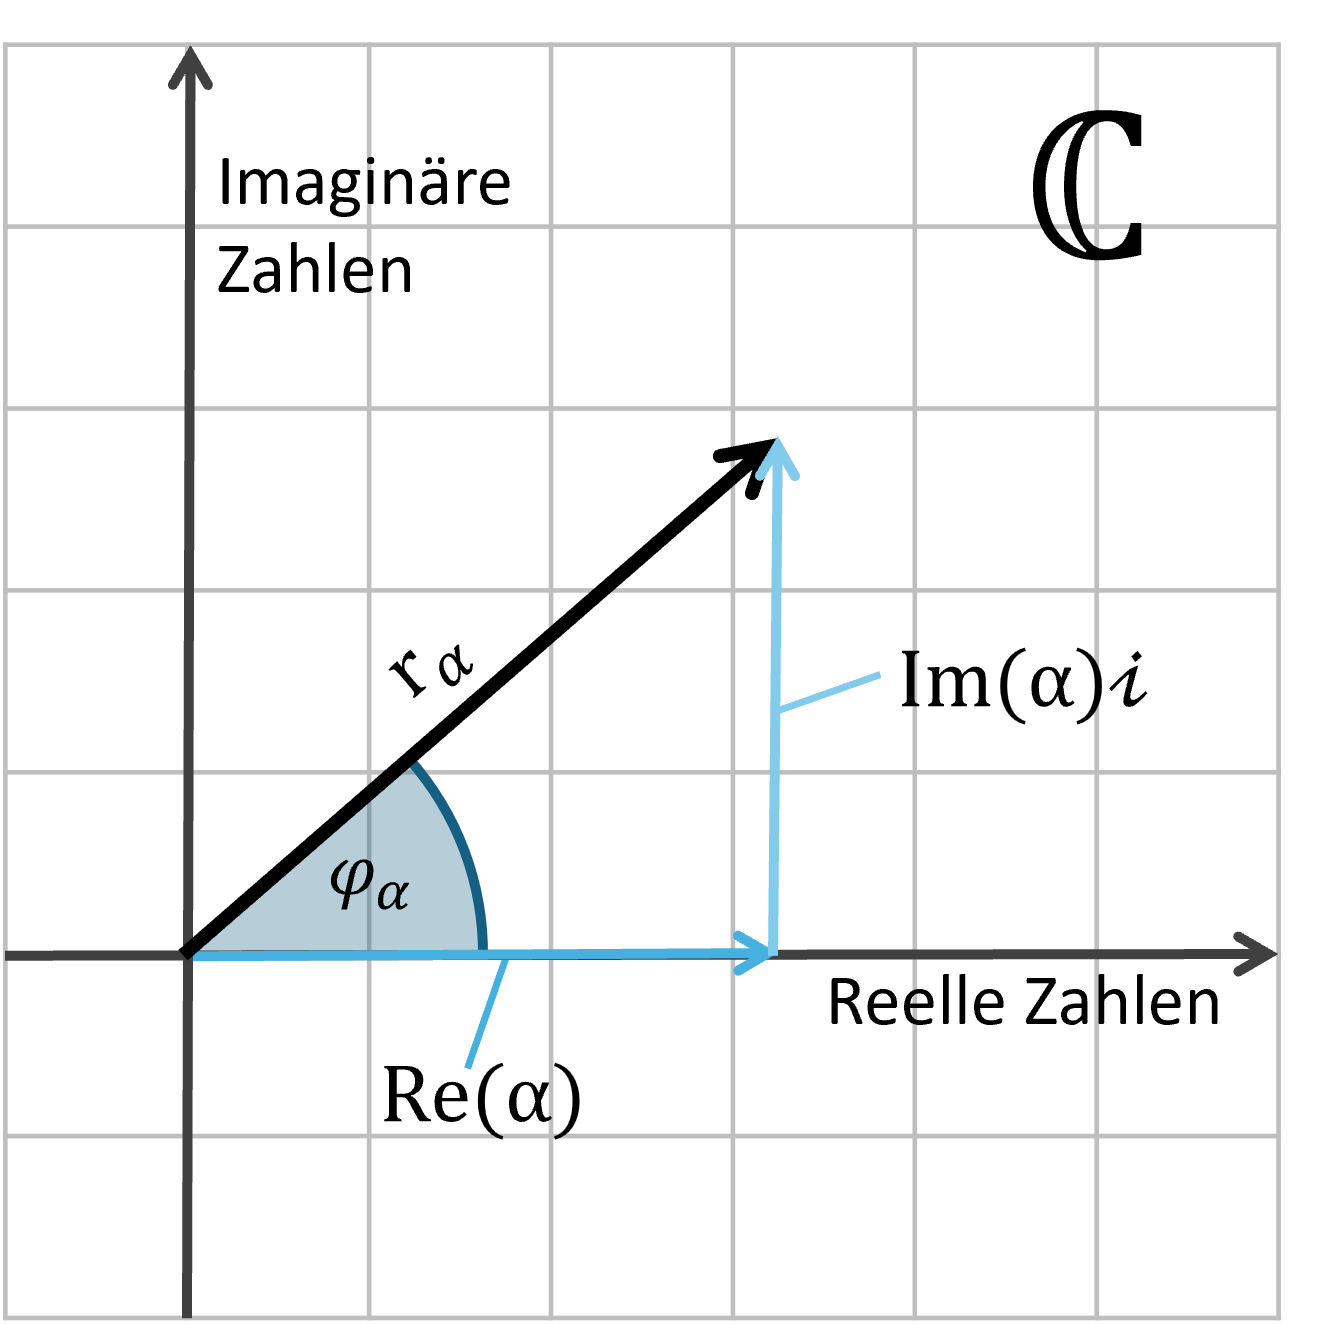
\includegraphics[width=0.4\textwidth]{images/explanation_complex_numbers.png}
    \caption{Darstellung komplexer Zahlen in der komplexen Ebene.}
    \label{fig:komplexe-zahlen}
    \end{figure}

    \item[\hypertarget{landau-notation-def}{}Landau-Notation]
    Eine mathematische Notation zur Analyse der Laufzeit von Algorithmen.
    Sie gibt an, wie schnell eine Funktion wächst, wenn die Eingabegrösse gegen unendlich geht.
    Zum Beispiel bedeutet \( O(n^2) \), dass die Laufzeit eines Algorithmus im schlimmsten Fall proportional zum Quadrat der Eingabegrösse \( n \) wächst \cite{landauNotation}.

    \item[\hypertarget{modulo-def}{}Modulo]
    Eine mathematische Operation, die den Rest einer Division zweier Zahlen angibt. Zum Beispiel ist \( 7 \mod 3 = 1 \) (oder auch geschrieben $ 7 \; \% \; 3 = 1 $), da 7 : 3 = 2 mit einem Rest von 1 ergibt.

    \item[\hypertarget{polynomialtime}{}Polynomzeit]
    Ein Polynom ist eine mathematische Funktion der Form \( P(n) = a_k n^k + a_{k-1} n^{k-1} + ... + a_1 n + a_0 \), wobei \( a_i \) Konstanten sind und \( k \) eine natürliche Zahl ist.
    Ein Polynom wächst also nicht exponentiell, sondern in einem viel langsameren Tempo.
    Ein Algorithmus läuft in Polynomzeit, wenn seine Laufzeit durch ein Polynom in Bezug auf die Eingabegrösse \( n \) beschrieben werden kann, also \( O(n^k) \) für einen konstanten Exponent \( k \).
    
    \item[\hypertarget{xor-gate-def}{}XOR-Gatter] 
    Ein logisches Gatter, das zwei Eingänge hat und genau dann eine 1 ausgibt, wenn die Anzahl der Eingänge mit dem Wert 1 ungerade ist.
    
    \begin{center}
    \begin{tabular}{|c|c|c|}
    \hline
    A & B & A XOR B \\
    \hline
    0 & 0 & 0 \\
    \hline
    0 & 1 & 1 \\
    \hline
    1 & 0 & 1 \\
    \hline
    1 & 1 & 0 \\
    \hline
    \end{tabular}
    \end{center}

\end{description}
\pagebreak
\section{Abkürzungsverzeichnis}
\begin{description}
    \item[FPGA] Field-Programmable Gate Array (feldprogrammierbare Gatter-Anordnung)
    \item[NIST] National Institute of Standards and Technology
    \item[QFT] Quanten-Fourier-Transformation
    \item[Qubit] Quantenbit
    \item[RSA] Rivest-Shamir-Adleman
    \item[PQC] Post-Quanten-Kryptographie
\end{description}

\section{Abbildungsverzeichnis}
\listoffigures

\section{Tabellenverzeichnis}
\listoftables
\pagebreak
\section{Literaturverzeichnis}
% Hier werden alle verwendeten Quellen aufgeführt, sowohl gedruckte als auch digitale Literatur.
% Literaturverzeichnis in Reihenfolge des Erscheinens im Text
\printbibliography[heading=none]

\pagebreak
\subsection{Mündliche Quellen}

\section*{Interview mit Dipl.-Ing. Christian Weber (WEEI) MBA}
Das Interview wurde am 27. Oktober 2025 telefonisch geführt.\vspace{1em}\\
\textit{Welche Verschlüsselungsverfahren wären Ihrer Einschätzung nach am stärksten bedroht, 
wenn morgen ein leistungsfähiger Quantencomputer verfügbar wäre?}\\
Grundsätzlich wären alle heute eingesetzten Verschlüsselungsverfahren betroffen. 
Nahezu sämtliche aktuell verwendeten kryptografischen Algorithmen gelten im Prinzip als bedroht, 
da es derzeit kein in der Praxis breit eingesetztes, vollständig quantensicheres Verfahren gibt. 
Zwar existieren bereits erste quantensichere Algorithmen, die auch auf klassischer Hardware lauffähig sind, 
diese befinden sich jedoch noch nicht im produktiven Einsatz, sondern überwiegend im Forschungs- 
oder Laborumfeld. Kritische Infrastrukturen wie Online-Banking-Systeme operieren nicht im Labor, 
sondern in realen, global vernetzten Umgebungen.
\vspace{1em}
\\
\hypertarget{pqc_security}{}\textit{Was versteht man unter quantensicheren Algorithmen und wie unterscheiden sie sich von 
klassischen Verschlüsselungsverfahren?}\\
Unter quantensicheren Algorithmen versteht man kryptografische Verfahren, die so aufgebaut sind, 
dass selbst ein Quantencomputer sie nicht in einer praktikablen Zeit brechen kann, auch nicht durch 
Brute-Force-Angriffe. Verschlüsselung zielt grundsätzlich nicht auf ewige Sicherheit ab, sondern darauf, 
Daten so lange zu schützen, bis sie ihren Wert verlieren. Dieses Prinzip gilt sowohl für klassische 
als auch für quantensichere Verfahren. Der wesentliche Unterschied liegt in der mathematischen Grundlage, 
da Quantencomputer völlig anders arbeiten als klassische von-Neumann-Rechner und deshalb neue Konzepte 
erfordern.
\vspace{1em}
\\
\hypertarget{pqc_migration}{}\textit{Welche konkreten Schritte werden derzeit unternommen, um digitale Systeme auf die Zeit 
leistungsfähiger Quantencomputer vorzubereiten?}\\
Aktuell werden vor allem Standardisierungsbemühungen in internationalen Arbeitsgruppen verfolgt. 
Ein koordinierter, staatlich gesteuerter Ansatz ist jedoch kaum erkennbar. Es existieren keine 
umfassenden Analysen nationaler Infrastrukturen hinsichtlich quantenbedingter Risiken. Besonders 
problematisch ist dies in Bereichen wie dem Gesundheitswesen, in denen grosse Mengen sensibler Daten 
gespeichert werden. Auf politischer Ebene ist das Thema bislang nur unzureichend angekommen.
\vspace{1em}
\\
\hypertarget{dependency_cryptography}{}\textit{Welche Branchen oder Institutionen wären besonders betroffen, wenn heutige Verschlüsselung 
plötzlich unsicher würde?}\\
Betroffen wären praktisch alle Bereiche. Banken sind aufgrund finanzieller Interessen besonders 
attraktive Ziele, ebenso blockchainbasierte Systeme. Das Militär wäre massiv betroffen, da moderne 
Waffensysteme vollständig auf verschlüsselter Kommunikation basieren. Auch Krankenhäuser, 
Verwaltungen und Unternehmen wären stark eingeschränkt, sobald öffentliche Netze genutzt werden. 
Sobald Verschlüsselung nicht mehr zuverlässig funktioniert, entsteht ein erhebliches Sicherheitsrisiko.
\vspace{1em}
\\
\hypertarget{longterm_security}{}\textit{Wie gross schätzen Sie die Gefahr ein, dass heute verschlüsselt gespeicherte Daten in Zukunft 
nachträglich entschlüsselt werden?}\\
Diese Gefahr ist aus meiner Sicht sehr hoch und liegt langfristig nahezu bei hundert Prozent. Schon 
heute lassen sich viele Verschlüsselungsverfahren mit ausreichend Zeit und Rechenleistung brechen. 
Ein leistungsfähiger Quantencomputer würde diesen Prozess erheblich beschleunigen. Besonders für 
Geheimdienste, aber auch für wirtschaftliche Analysen, sind historische Daten von grossem Interesse, 
da sich daraus zukünftige Entwicklungen ableiten lassen.
\vspace{1em}
\\
\textit{Welche gesellschaftlichen Folgen hätte es, wenn persönliche Daten oder staatliche Geheimnisse 
plötzlich offenlägen?}\\
Einzelne Datenlecks führen erfahrungsgemäss nur zu geringen gesellschaftlichen Reaktionen. 
Kritisch wird es jedoch, wenn ganze digitale Systeme nicht mehr zuverlässig funktionieren. Elektronische 
Identitäten, digitale Gesundheitsdaten oder bargeldloser Zahlungsverkehr könnten ausfallen. Ohne 
funktionierende Ersatzverfahren wären Staaten, Unternehmen und Gesundheitssysteme erheblich 
eingeschränkt. Die Auswirkungen wären vergleichbar mit einem grossflächigen Stromausfall.
\vspace{1em}
\\
\textit{Könnte ein Wettlauf um die Quantencomputerüberlegenheit zu globalen Machtverschiebungen führen, 
vergleichbar mit der Entwicklung von Atomwaffen?}\\
Ja, eindeutig. Wer im Bereich des Quantencomputings führend ist, erlangt erhebliche wirtschaftliche, 
technologische und militärische Vorteile. Quantencomputer ermöglichen extrem schnelle Datenanalyse, 
Optimierung und Simulation. Diese Fähigkeiten können sowohl zivil als auch militärisch eingesetzt 
werden und bergen ein erhebliches strategisches Potenzial.
\vspace{1em}
\\
\hypertarget{overall_security}{}\textit{Glauben Sie, dass die Gesellschaft rechtzeitig auf eine Ära leistungsfähiger 
Quantencomputer vorbereitet sein wird?}\\
Nein, als Gesellschaft sind wir darauf nicht ausreichend vorbereitet. Es fehlt an grundlegender 
technologischer Bildung und an einem Verständnis für Schlüsseltechnologien. Bereits in der Schule 
sollte ein Basiswissen über digitale Systeme, IT-Sicherheit und neue Technologien vermittelt werden. 
Viele Menschen nutzen diese Systeme, ohne ihre Funktionsweise oder Risiken zu verstehen, was langfristig 
zu Abhängigkeiten und Fehlentscheidungen führen kann.
